
\section{Overview of Heavy-Tailed Self-Regularization}
\label{sxn:theory-review}

%In this section, we will briefly review results from Universality that will be relevant for our analylsis.
s s review Martin and Mahoney's Theory of Heavy-Tailed Self-Regularization (HT-SR)~\cite{MM18_TR}.
%%\michael{We need to push the other 10 pager to the archive, without the supplementary information}

Write the Energy Landscape (or optimization function) for a typical DNN with $L$ layers, with activation functions $h_{l}(\cdot)$, and with $N\times M$ weight matrices $\mathbf{W}_{l}$ and biases $\mathbf{b}_{l}$, as follows:
\begin{equation}
E_{DNN}=h_{L}(\mathbf{W}_{L}\times h_{L-1}(\mathbf{W}_{L-1}\times h_{L-2}(\cdots)+\mathbf{b}_{L-1})+\mathbf{b}_{L})  .
\label{eqn:dnn_energy}
\end{equation}
%WLOG,
Typically, this model would be trained on some labeled data $\{d_{i},y_{i}\}\in\mathcal{D}$, using Backprop, by minimizing the loss $\mathcal{L}$.
For simplicity, we do not indicate the structural details of the layers (e.g., Dense or not, Convolutions or not, Residual/Skip Connections, etc.). 
Each layer is defined by one or more layer 2D weight matrices $\mathbf{W}_{l}$, and/or the 2D feature maps $\mathbf{W}_{l,i}$ extracted from 2D Convolutional (Conv2D) layers.
(We have not yet analyzed LSTM or other complicated Layers.) 
A typical modern DNN may have anywhere between 5 and 5000 2D $\mathbf{W}_{l,i}$ layer matrices.%
\footnote{%
%Some notational conventions:
For each Linear Layer, we get a  single $(N\times M)$ (real-valued) 2D weight matrix, denoted $\mathbf{W}_{l}$, for layer $l$.  
This includes Dense or Fully-Connected (FC) layers, as well as 1D Convolutional (Conv1D) layers, Attention matrices, etc.
We ignore the bias here terms $\mathbf{b}_{l}$ in this analysis. 
%XXX.  WHY, WHAT.   
Let the aspect ratio be $Q=\frac{N}{M}$, with $Q\ge 1$.
For the Conv2D layers, we have a 4-index Tensor, of the form $(N\times M \times c\times d)$, consisting
of $c\times d$ 2D feature maps of shape $(N\times M)$.    
We  extract $n_{l}=c\times d$ 2D weight matrices $\mathbf{W}_{l,i}$, one for each feature map $i=[1,\dots,n_{l}]$ for layer $l$.
%One could construct matrices in other ways.
}
   

\paragraph{Heavy-Tailed Empirical Spectral Distributions.}
%
%By Universal behavior, we mean that the eigenvalue spectrum associated weight matrices 
%We can identify different Universality classes 
%
In the HT-SR Theory, we analyze the eigenvalue spectrum (the ESD) of the associated correlation matrices~\cite{MM18_TR}.
From this, we can characterize the amount and form of correlation, and therefore implicit self-regularizartion, present in the DNN's weight matrices.
For each layer weight matrix, $\mathbf{W}_{l}$, construct the associated $M\times M$ (uncentered) correlation matrix $\mathbf{X}$. 
Dropping the $L$ and $l,i$ indices, we have
$$
\mathbf{X} = \frac{1}{N}\mathbf{W}^{T}\mathbf{W}.
$$
%In theoretical treatments, $\gamma$ depends on the form of $\Probab{W_{i,j}}$, e.g., the value of $\mu$, in order to prove the existence of the limiting forms of the ESD.
%For MP theory and the Gaussian Universality class, we can set $\gamma=1$, but for the HT Universality classes, we need to set $\gamma=2/\mu$.
%Of course, empirically, we do not know the PL exponent $\mu$, or the particular Universality class, \emph{a priori}, and the data are of only finite size.
%This will be very important below. 
%For our empirical analysis, we set $\gamma=1$ and deal with these issues in an \emph{a posteriori} manner. 
%
If we compute the eigenvalue spectrum of $\mathbf{X}$, i.e.,
$  % $$
\mathbf{X}\mathbf{v}_{i}=\lambda_{i}\mathbf{v}_{i} , 
$  % $$
then the ESD of eigenvalues, $\rho(\lambda)$, is just a histogram of the eigenvalues, formally written as
\begin{equation}
\rho(\lambda)=\sum\limits_{i=1}^{M}\delta(\lambda-\lambda_{i})  .
\label{eqn:eigenval_hist}
\end{equation}
%
%From HT-RMT theory~\cite{XXX-XXX,XXX-XXX,XXX-XXX,XXX-XXX}, the ESD $\rho(\lambda)$ of a HT matrix will have a HT, taking the form
Empirically, for weight matrices of a modern well-trained production-quality DNN, the ESD nearly always exhibits Heavy-Tailed properties~\cite{MM18_TR}.%
\footnote{Older and smaller models exhibit ESD properties closer to a Spiked Covariance model, and it is possible to train DNNs to have ESDs with other properties, corresponsing to other types of implicit self regularization~\cite{MM18_TR}.} 
Using HT-SR Theory, we can characterize the \emph{correlations} in a weight matrix by examining its ESD, $\rho(\lambda)$.
It can be well-fit to a power law (PL) distribution, given as
\begin{equation}
\rho(\lambda)\sim\lambda^{-\alpha}  ,
\label{eqn:eigenval_pl}
\end{equation}
which is (at least) valid within a bounded range of eigenvalues $\lambda\in[\lambda_{min},\lambda_{max}]$.  
%\michael{Ques: here, $\alpha$ is theoretical, while below $\alpha$ is fit, so clarify.}
%
We can determine $\alpha$ by fitting the   ESD to a PL, using the commonly accepted Maximum Likelihood (MLE) method of Clauset et al.~\cite{CSN09_powerlaw,ABP14}.
%(((
%\charles{Discuss fact the PL tails are Frechet at finite-size so only need to fit the bulk}
%\michael{Ques: clarify.}
%)))
This method works very well for exponents between $\alpha\in(2,4)$, and it is adequate, although imprecise, for smaller and larger $\alpha$~\cite{newman2005_zipf}. 
%\michael{Ques: careful, $\alpha$ (thoeretical or fitted) or $\mu$ here.}
%%MM%% The fitting method is robust in that it is reasonably insensitive to the the choice of normalization $\gamma=1$.

%% %Recent work by Martin and Mahoney
%% in our previous study of Heavy-Tailed Self Regularization (HT-SR)~\cite{MM18_TR}, we examine the eigenvalue density
%% $\rho(\lambda)$, or Empirical Spectral  Density (ESD), of the linear weight matrices of very large number of modern, pre-trained, DNNs,
%% such as the AlexNet, the VGG series (VGG11, VGG13, ...) ,  etc. 

\charlesX{comments  will go back in}
%% \charlesX{
%% We apply our new Theory of Heavy-Tailed Self Regularization (HT-SR) to analyze these large, pre-trained DNNs.  
%% We model \emph{the correlations} arising in the DNN layers by forming the normalized correlation matrices $\mathbf{X}=(1/N)\mathbf{W}_{L}^{T}\mathbf{W}_{L}$ 
%% for each of the individual  the layer weight matrices $\mathbf{W}_{L}$ and then studying the eigenvalue density of each $\mathbf{X}$,  $\rho(\lambda)$.
%% The HT-SR Theory lets us characterize the densities because they almost always display heavy tailed signatures,
%%  and can be fit to a Power Law, $\rho(\lambda)\sim\lambda^{-\alpha}$, with exponent $\alpha$.   And , on average,
%%  the smaller the $\alpha$, the more Self Regularization is in the DNN.  Of course, the
%%   pre-trained weight matrices  $\mathbf{W}_{L}$  themselves are not at all random because they have been trained 
%%   on very large, high quality data sets,
%%   and they behave quite differently from a random heavy tailed (i.e. Pareto) matrix.  And it is these differences we can exploit
%%   to predict trends in the generalization accuracy.}

The original work on HT-SR Theory~\cite{MM18_TR} considered NNs including AlexNet and InceptionV3 (as well as DenseNet, ResNet, and VGG), and it showed that for nearly every $\mathbf{W}$, the (bulk and tail) of the ESDs can be fit to a PL and the PL exponents $\alpha$ nearly all lie within the range $\alpha\in(1.5,5)$.
Moreover, smaller exponents appear $\alpha$ are correlated with more self-regularization and, correspondingly, better generalization~\cite{MM18_TR}.
Subsequent work~\cite{MM18_unpub_work} has shown that these results are ubiquitous. 
%\michael{Put ref to notebook in~\cite{MM18_unpub_work}.}
In particular, upon examining nearly 10,000 layer weight matrices $\mathbf{W}_{l,i}$ across over 50 different modern pre-trained DNN architectures, the ESD of nearly every $\mathbf{W}$ layer matrix can be fit to a PL:
$70-80\%$ of the time, the fitted PL exponent $\alpha$ lies in the range $\alpha\in(2,4)$; and  %% (in the Moderately Heavy-Tailed Universality class, described below); and
$10-20\%$ of the time, the fitted PL exponent $\alpha$ lies in the range $\alpha< 2$.  %% (in the Very Heavy-Tailed Universality class, described below).
For example, see Figure~\ref{fig:power-law-histogram} for a histogram of results for ca. 7500 weight matrices from ImageNet.
%\charlesX{explain this plot, ref to notebook and check in.  This plot is for ImageNet, includes conv@D feature maps, lots of small alpha, but not as good a fit.}
Of course, there are exceptions: in any real DNN, the fitted $\alpha$ may range anywhere from $\sim 1.5$ to $10$ or higher~\cite{MM18_unpub_work}.  

\begin{figure}[t] %[!htb]
   \centering
   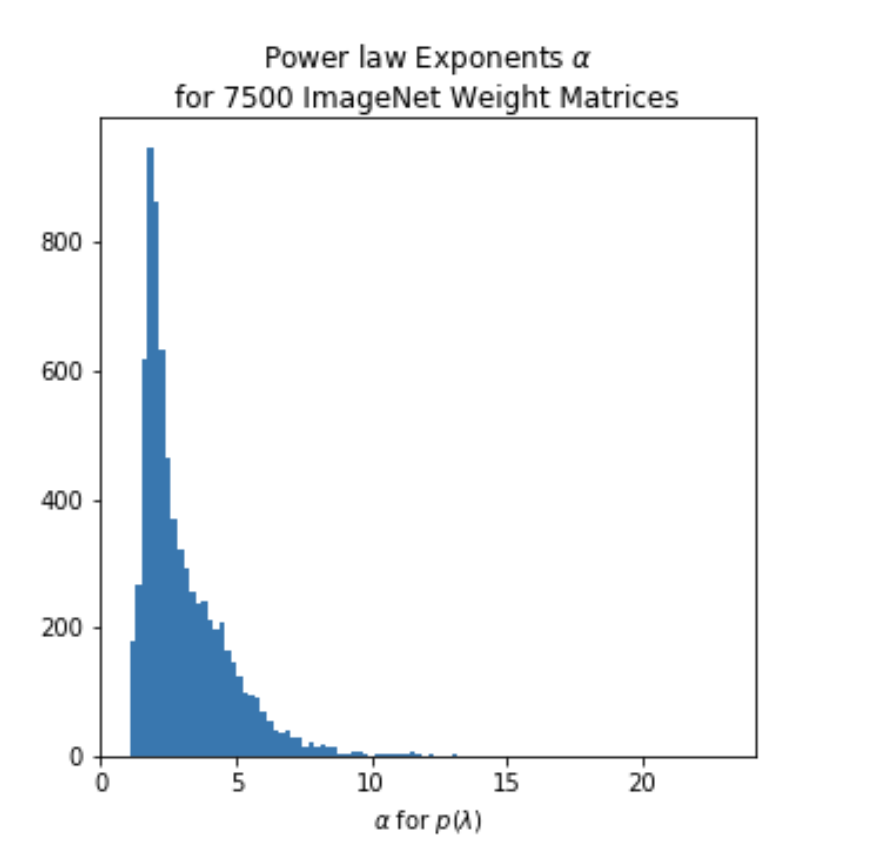
\includegraphics[scale=0.40]{img/power-law-histogram.png} 
   \caption{Histogram of fitted PL exponents $\alpha$ for ca. 7500 Linear and Conv2D Layers from ImageNet.  The vast majority have $\alpha\in(1.5,5)$.  Some Conv2D layers have smaller values of $\alpha$; and larger values of $\alpha$ (up to ca. 20) exist but correspond to less reliable fits. \michael{Charles, zoom in on X axis for fig, so don't go above 10.} }
   \label{fig:power-law-histogram}
\end{figure}




%\nred{removed this: \paragraph{Simple Random Matrix Models.} }
%One might imagine that the matrix elements of $\mathbf{W}$ are drawn from some probability distribution, e.g., a Normal $N(0,\sigma)$ distribution
%\begin{equation}
%\Probab{ W_{i,j} } \sim N(0,\sigma)
%\end{equation}
%with mean $0$ and variance $\sigma$.%
%\footnote{At the start of training, DNN weight matrices typically are approximately Normal.  This has been used by some as an analytically-tractable model for trained DNNs, but it is an empirical question whether this is a good model for very non-random matrices that arise at the end of training modern DNNs.  Empirically, it is not~\cite{MM18_TR}.}
%%MM%% \charlesX{Our imagination here lets us derive seemingly \emph{Universal} expressions for how the correlations should behave, even though $\mathbf{W}$  itself is not at all random. }
%These Gaussian models arise in the well known Marchenko-Pastur (MP) RMT~\cite{XXX-XXX}, as well as the Spiked-Covariance model~\cite{johnstone2009}, which is a perturbative variant of MP-RMT. 
%Empirically, it is know that these Gaussian-based models are useful for understanding older, smallish Neural Networks, such as LeNet5~\cite{MM18_TR}.
%More modern DNNs, however, display very different, more exotic,  Universal, behavior.  


\paragraph{Heavy-Tailed Universality.} 

Due to the training process, trained DNN weight matrices are strongly-correlated; and fitting their ESDs to Eqn.~(\ref{eqn:eigenval_pl}) amounts to \emph{modeling} the correlational properties in terms of known HT Universality classes~\cite{SornetteBook,BouchaudPotters03}.
In statistics and applied mathematics, Universality typically refers to properties of systems that can be modeled by random matrices (the justification being that certain system properties can be deduced, without requiring knowledge of the system details, from a few global quantities that are then used as parameters to define a random matrix ensemble)~\cite{ER05,EW13}.
In Statistical Physics, on the other hand, Universality is \emph{used} to construct scaling relations (that are then empirically evaluated) between empirically-measurable quantities~\cite{SornetteBook,BouchaudPotters03}. 
In this case, random matrices arise since they are particularly easy-to-analyze members of a Universality class, for which these relations should hold.
In particular, strongly-correlated DNN weight matrices are clearly not random matrices, but the latter can be used to \emph{model} the former (since, if they are members of the same Universality class, then scaling relations should hold for both).
See Figure~\ref{fig:universality_diagram} for an illustration.
We use HT-RMT and Universality in the way used in Statistical Physics, i.e., to derive Universal relations between empirically-measurable~quantities.

%% \charles{%
%% EXPLAIN UNIVERSALITY, AS WE USE IT, IN THIS SECTION. 
%% NOTE: we model the ESD of X, the correlations in W, and therefore how the data has been learned. 
%% Universality of Power Law exponents is special, in the context of statistical physics / Rg theory / SOC, and different from Universality in RMT. 
%% We use RMT as a guide.
%% This section contains LOTS OF NEW information, including the 2 images and the discussion around them. 
%% Notice: the conv2D maps are VHT, not MHT.
%% So we will need an approach that crosses the 2 Universality classes. 
%% Notice: W is not itself random, but its ESD lookd like the ESD of an HT RMT.}

\begin{figure}[t]  %[!htb]
   \centering
   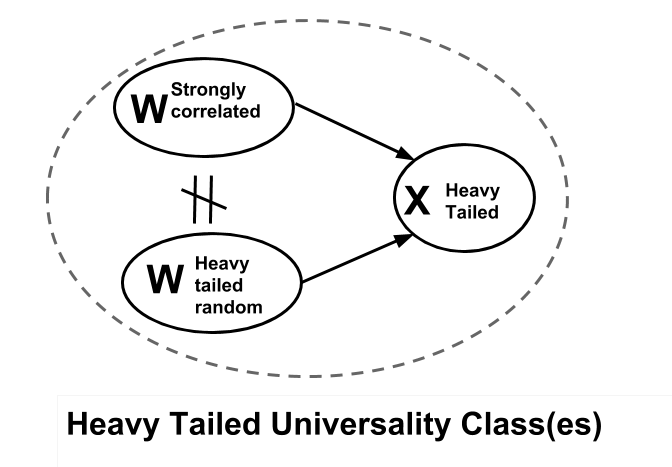
\includegraphics[scale=0.40]{img/universality_classes.png} 
   \caption{Illustration of our use of HT Universality.  
            \michael{Charles, maybe tweak this figure to rotate and horizontally show transfer of Universal things between different matrices.}  
            A random matrix $\mathbf{W}(\mu)$ with elements drawn i.i.d. from the HT distribution of Eqn.~(\ref{eqn:ht_dstbn}) and weight matrix from a modern well-trained DNN that exhibits strong correlations $\mathbf{W}^{str. corr.}$ each arise from different generative mechanisms, and they different.  Both exhibit similar Universality properties, as evidneced by the HT properties of the ESDs of their corresponding correlation matrices $\mathbf{X}$, and so we expect Universal properties to be similar between them.}
   \label{fig:universality_diagram}
\end{figure}


\paragraph{Heavy-Tailed Random Matrix Theory.} 
To characterize this behavior, we use a HT variant of RMT, where we use HT random matrices to elucidate different Universality classes.
Let $\mathbf{W}(\mu)$ be an $N \times M$ random matrix with entries chosen i.i.d. from
\begin{equation}
\Probab{ W_{i,j} } \sim \dfrac{W_{0}^{\mu}}{|W_{i,j}|^{1+\mu}}  ,
\label{eqn:ht_dstbn}
\end{equation}
where $W_{0}$ is the typical order of magnitude of $W_{i,j}$, and where $\mu>0$. 
These HT matrix models were first introduced in the Statistical Physics literature, where they are called \'L\'evy Matrices when $0<\mu<2$~\cite{PB94}; see also~\cite{BM97,BJNx01_TR,BJNx06_TR,heavytails2007}.
More recently there has been more mathematical work on HT random matrices~\cite{AG08,AAP09,BJ09_TR,DPS14,AT16}.
There are at least 3 different Universality classes%
\footnote{Results for $\mu=2,4$ are slightly different~\cite{SornetteBook,BouchaudPotters03}.  We don't describe them since we don't expect to be able to resolve them numerically.  Also, sometimes L\'evy matrices are split into VHT for $1<\mu<2$ and EHT (Extremely Heavy-Tailed) for $0<\mu<1$, as the properties for these two parameter regimes are somewhat different~\cite{SornetteBook,BouchaudPotters03}.}
of Heavy-Tailed random matrices, defined by the range $\mu$ takes on:
\begin{itemize}
\item $0<\mu<2$: VHT: Universality class of Very Heavy-Tailed (or L\'evy) matrices;
\item $2<\mu<4$: MHT: Universality class of Moderately Heavy-Tailed (or Fat-Tailed) matrices;
\item $4<\mu$: WHT: Universality class of Weakly Heavy-Tailed matrices.
\end{itemize}
%%
%%\charles{ THIS SECTION REVIEWS Heavy Tail RMT, and is ALL REVIEW.  WE MUST  explain how to interpret a correlated ESD in terms of HT-RMT.  BUT be clear that this is not the whole story }
%%
%%\michael{We need to highlight how the HT Universality we use is one that crosses Universality classes, i.e., VHT and finite-sized MHT, and certainly is NOT limited to random matrices, but we use RMT to characterize certain things.}
%%


\paragraph{Heavy-Tailed, Finite-Size Relations.} 

\charlesX{Discuss empirical measurements, theoretical parameters, how to relate}

\charlesX{Lots removed ?}

'
\charlesX{NEED BETTER INTRO}




%% For the VHT Universality class, the PL tail of Eqn.~(\ref{eqn:eigenval_pl}) persists in the infinite limit $N\rightarrow\infty$, for $Q$ fixed; and
%% we have the linear relation between our observed exponent $\alpha$ and the theoretical~$\mu$:
%% \begin{equation}
%% \alpha=\frac{1}{2}\mu+1  .
%% \label{eqn:alpha_mu_vht}
%% \end{equation}
%% \michael{Ques: careful, two things change here: observed versus theoretical, and matrix elements versus eigenvalues.}
%% This expression which works very well at finite size, even for very small matrices $(M,N\approx100)$.
%% %
%% For the MHT Universality class, the PL tail of Eqn.~(\ref{eqn:eigenval_pl}) vanishes in the infinite limit $N\rightarrow\infty$, for $Q$ fixed.
%% \michael{Ques: what does ``vanishes'' mean, it changes slope, and it is MP in the limit for WHT.}
%% At all finite sizes, however, it persists, and it follows a Frechet distribution (i.e., an exponentially-truncated PL). 
%% Here, $\alpha$ is still linear in $\mu$, but it displays very strong finite-size effects, empirically giving 
%% \begin{equation}
%% \alpha=a\mu+b, 
%% \label{eqn:alpha_mu_mht}
%% \end{equation}
%% where $a,b$ depend strongly on $M,N$. 
%% (See Table 3 of \cite{MM18_TR} and Figure~\ref{XXX} below for more details on this.)
%% These strong finite-size effects characterize these MHT distributions; and they are well-known in the Statistical Physics literature~\cite{SornetteBook,BouchaudPotters03}. 
%% We will exploit these finite-size effects to develop our-theory.

For the VHT Universality class, the PL tail of Eqn.~(\ref{eqn:eigenval_pl}) persists in the infinite $N\rightarrow\infty$ limit, for $Q$ fixed; and
we have the linear relation between our observed exponent $\alpha$ and the theoretical~$\mu$:
%
\begin{subequations}
\label{eqn:alpha_mu_vht_and_mht}
\begin{align}
\text{VHT:}\;\;\;\alpha=\frac{1}{2}\mu+1  .
\label{eqn:alpha_mu_vht}
\end{align}
%% \michael{Ques: careful, two things change here: observed versus theoretical, and matrix elements versus eigenvalues.}
This asymptotic expression works very well at finite size, even for very small matrices $(M,N\approx100)$.
%
For the MHT Universality class, the PL tail of Eqn.~(\ref{eqn:eigenval_pl}) holds in the infinite $N\rightarrow\infty$ limit, for $Q$ fixed, for $\alpha$ in Eqn.~(\ref{eqn:alpha_mu_vht}).
At all finite sizes, however, $\alpha$ is still linear in $\mu$, but it displays \emph{very} strong finite-size effects, empirically giving 
\begin{align}
\text{MHT:}\;\;\;\alpha=a\mu+b, 
\label{eqn:alpha_mu_mht}
\end{align}
\end{subequations}
%
where $a,b$ depend strongly on $M,N$. 
(See Table 3 of \cite{MM18_TR} and Figure~\ref{fig:randW} below for more details.)
These strong finite-size effects characterize MHT distributions; and they are well-known in Statistical Physics~\cite{SornetteBook,BouchaudPotters03}. 
We will exploit these finite-size effects to develop our-theory.

Finally, for both the VHT and the MHT Universality classes, the maximum empirical eigenvalue, $\lambda_{max}$, follows a Frechet distribution (i.e., an exponentially-truncated PL); and we expect it to scale with $N$ according to Extreme Value Theory (EVT)~\cite{heavytails2007,disordered2007,Resnick07,MM18_TR}:
\begin{equation}
\text{VHT\;\&\;MHT:}\;\;\;\lambda_{max}\sim N^{4/\mu-1}  
\label{eqn:scaling_of_lambda_max}
\end{equation}
(where, for simplicity, $Q=1$).
\michael{MM ques: do we make $Q$ dependence explicit here and elsewhere.}
Importantly, \emph{due to HT Universality}, we expect Eqn.~(\ref{eqn:scaling_of_lambda_max}) to hold for matrices in these HT Universality classes (as evidenced by their ESD properties), e.g., DNN weight matrices $\mathbf{W}$ after training, \emph{even when the matrix is not itself a HT random matrix} and therefore not governed by~EVT.
\michael{MM ques: maybe derive these 2 relations---Eqns.~(\ref{eqn:alpha_mu_vht_and_mht}) and~(\ref{eqn:scaling_of_lambda_max})---in the appendix.}


\charlesX{AWKWARD point sentence}

Let's clarify Eqns.~(\ref{eqn:alpha_mu_vht_and_mht}) and~(\ref{eqn:scaling_of_lambda_max}):  
$\alpha$ and $\lambda_{max}$ are empirically-measurable quantities (of real or synthetic matrices), while $\mu$ is a parameter of theory (in particular, of HT-RMT).
Eqns.~(\ref{eqn:alpha_mu_vht_and_mht}) and~(\ref{eqn:scaling_of_lambda_max}) show that we have very simple relationships that apply to random matrices that lie within both the VHT and MHT Universality classes.
Our goal will be to use this to derive a relationship that holds between $\alpha$, $\lambda_{max}$, and perhaps other observables such as matrix norms, and then appeal to HT Universality to apply it to non-random pre-trained DNN weight matrices that also lie within these HT Universality classes.

%\section{Using Heavy-Tailed Universality}
%\section{Relating Heavy-Tailed Universality to Capacity Metrics}
\section{Heavy-Tailed Universality and Capacity Control Metrics}
\label{sxn:theory-new}

%In this section, we will describe our proposed capacity control metric.
%
From prior work~\cite{MM18_TR}, we expect that smaller PL exponents of the ESD imply more regularization and therefore better generalization. 
Since smaller norms of weight matrices often correspond to better capacity control~\cite{LMBx18_TR,SHNx17_TR,PLMx18_TR,BFT17_TR}, we would like to relate the empirical PL exponent $\alpha$ to the empirical Frobenius norm $\Vert\mathbf{W}\Vert_{F}$.
At least na\"{\i}vely, this is a challenge, since smaller PL exponents often correspond to larger matrix norms (and thus worse generalization).
To resolve this apparent discrepancy, we will exploit HT Universality to propose a Universal DNN complexity metric.


\paragraph{Form of a Proposed Universal DNN Complexity Metric.} 

The PL exponent $\alpha$ is a complexity metric for a single DNN weight matrix, with smaller values corresponding to greater regularization~\cite{MM18_TR}.
% The fitted PL  ... AWK
It describes how well that matrix encodes complex correlations in the training data.
Thus, a natural class of complexity or capacity metrics to consider for a DNN is to take a \emph{weighted average}%
\footnote{There are several reasons we don't want a simple unweighted average: an unweighted average behaves differently for HT random matrices than for well-trained DNN weight matrices, and so it would not be Universal; we want a metric that relates the $\alpha$ of HT-SR Theory with known capacity control metrics such as norms of weight matrices, and including weights permits this flexibility; and unweighted averages, while sometimes providing predictive quality, do not perform as reliably well. }
of the PL exponents, $\alpha_{l,i}$, for each layer weight matrix $\mathbf{W}_{l,i}$:
\begin{equation}
\hat{\alpha}:=\dfrac{1}{N_L}\sum_{l,i}b_{l,i}\alpha_{l,i}  .
\label{eqn:alpha_hat_generic}
\end{equation}
Here, the smaller $\hat{\alpha}$, the better we expect the DNN to represent training data, and (presumably) the better the DNN will generalize to new data.
The question is: what are good weights~$b_{l,i}$?

As we now show, we can extract the weighted average $\hat{\alpha}$ directly from the more familiar Product Norm, by exploiting both HT Universality, and its finite-size effects, arising
in DNN weight matrices.


%%%\paragraph{THEOREM:} \emph{The data dependent VC-like complexity of a Deep Neural Network can be expressed a weighted average the of power law exponents describing the empirical spectral density of the layer weight matrices}
%%
%%%\charles{\paragraph{PROOF:...}}


\paragraph{Product Norm Measures of Complexity.} 

%% XXX. I PUT THIS MOSTLY IN THE INTRO.
%% \charlesX{NEED TO CLARIFY 
%% Worst case Bounds vs Average Case for complexity metrics, and REVIEW MORE OF HIDary's work, either here and/or in the Intro}
%% \michael{Their method works well on toy data for worst-case, and to get it to work they need to modify the loss function in worse-case, but if we consider average case then we can apply it to large realistic DNNs---put these comments here or in intro.}

It has been suggested that the complexity, $\mathcal{C}$, of a DNN can be characterized by the product of the norms of the layer weight matrices,
$$
\mathcal{C}\sim\Vert\mathbf{W}_{1}\Vert\times\Vert\mathbf{W}_{2}\Vert\cdots\Vert\mathbf{W}_{L}\Vert ,
$$
where $\Vert\mathbf{W}\Vert$ is, e.g., the Frobenius norm~\cite{LMBx18_TR, SHNx17_TR,PLMx18_TR}.%
\footnote{Here, we can use either $\Vert\mathbf{W}\Vert$ or $\Vert\mathbf{W}\Vert^{2}$, and one can view $\mathcal{C}$ as akin to a data-dependent VC complexity.}
To that end, we consider a log complexity
\begin{eqnarray*}
\log\mathcal{C} &\sim& \log\bigg[\Vert\mathbf{W}_{1}\Vert\times\Vert\mathbf{W}_{2}\Vert\cdots\Vert\mathbf{W}_{L}\Vert\bigg]  \\
                &\sim& \bigg[\log\Vert\mathbf{W}_{1}\Vert+\log\Vert\mathbf{W}_{2}\Vert\cdots\log\Vert\mathbf{W}_{L}\Vert\bigg]  ,
\end{eqnarray*}
and we define the average log norm of the weight matrices as
\begin{equation}
\langle\log\Vert\mathbf{W}\Vert\rangle=\dfrac{1}{N_{L}}\sum_{l}\log\Vert\mathbf{W}_{l}\Vert  .
\label{eqn:av_log_norm}
\end{equation}

%% \michael{Ques: is the notation for layers or convolutions or what, be consistent with Eqn.~(\ref{eqn:alpha_hat_generic}).}
%% \charlesX{Need more references to Hidary's work}
%% MM: A BIT HERE, BUT MOST IS IN INTRO AND CONCLUSION.


\paragraph{A Universal, Linear, PL--Norm Relation.} 

We propose a simple linear relation between the (squared) Frobenius norm $\Vert\mathbf{W}\Vert^{2}_{F}$ of $\mathbf{W}$, the PL exponent $\alpha$, and the maximum eigenvalue $\lambda_{max}$ of $\mathbf{X}$ (i.e., the spectral norm $\Vert\mathbf{X}\Vert_{2}=\frac{1}{N}\Vert\mathbf{W}\Vert^{2}_{2}$):  
\begin{equation}
\textbf{PL--Norm Relation:} \quad \alpha\log\;\lambda_{max}\approx\log\;\Vert\mathbf{W}\Vert^{2}_{F}  .
\label{eqn:basic_relation}
\end{equation}
To our knowledge, this is the first time this PL--Norm relation has been noted in the literature (although prior work has considered norm bounds for HT data~\cite{MN09_TR}).
A few comments on Eqn.~(\ref{eqn:basic_relation}).
First, it provides a connection between the PL parameter $\alpha$ of HT-SR Theory and the weight norm $\Vert\mathbf{W}\Vert^{2}_{F}$ of more traditional statistical learning theory.
Second, it has the form of the well-known Hausdorff dimension~\cite{Sch07}.
Third, it shows that the fitted PL exponent can alternatively be interpreted as (up to the $\frac{1}{N}$ scaling) approximately the Stable Rank in Log-Units:
$$
\mbox{Log-Units Stable Rank:} 
\quad
\mathcal{R}^{log}_{s}:=\dfrac{\log\Vert\mathbf{W}\Vert^{2}_{F}}{\log\lambda_{max}}  \approx \alpha  .
$$
Our justification for proposing Eqn.~(\ref{eqn:basic_relation}) is three-fold.
%%\charles{GOOD}
\begin{enumerate}
\item
\label{enum:first}
We derive Eqn.~(\ref{eqn:basic_relation}) in the special case of very small PL exponent, $\alpha \rightarrow 1$, for an $N\times M$ random matrix $\mathbf{W}$ (with $N=M$, or $Q=1$, for simplicity).
\item
\label{enum:second}
We observe empirically that multiplying $\alpha$ by $\log\lambda_{max}$ leads to a relation that increases nearly linearly with $\log\Vert\mathbf{W}\Vert^{2}_{F}$ for a random HT matrix $\mathbf{W}$ and that is linearly correlated for real a DNN weight matrix $\mathbf{W}$. 
%This is precisely what we want for our simple HT-based complexity metric.
\item
\label{enum:third}
\emph{Based on Universality}, we expect this result to extend to larger exponents, both across the VHT Universality class, $\alpha\in(1,2)$, and into the \emph{finite-sized} MHT Universality class, $\alpha\in(2,4)$, where it applies for the finite-size weight matrices in DNNs.
\end{enumerate}
We will discuss each of these in more detail below.

Finally, based on Eqn.~(\ref{eqn:basic_relation}), we choose the weights in Eqn.~(\ref{eqn:alpha_hat_generic}) to be the log of the corresponding maximum eigenvalues of $\mathbf{X}$, i.e., for a given $l,i$, we have 
$$
b_{l,i} = {\lambda_{l,i}}_{max}  .
$$
Then, we define the complexity metrics for Linear and Convolutional Layers as follows:
%% $$
%% \text{Linear Layer:}\;\;\log\Vert\mathbf{W}_{L}\Vert^{2}_{F}\rightarrow\log\lambda^{max}_{L}\alpha_{L}  .
%% $$
%% \michael{Need to be consistent with superscripts and subscripts, on $\lambda$, in this par and elsewhere.}
%% $$
%% \text{Conv2D Layer:}\;\;\log\Vert\mathbf{W}_{L}\Vert^{2}_{F}\rightarrow \sum_{i=1}^{n_{L}}\log\lambda^{max}_{i,L}\alpha_{L,i}  .
%% $$
\begin{eqnarray*}
\text{Linear Layer:} & & \log\Vert\mathbf{W}_{l}\Vert^{2}_{F} \quad \rightarrow \quad \log{\lambda_{l}}_{max}\alpha_{l}  \\
\text{Conv2D Layer:} & & \log\Vert\mathbf{W}_{l}\Vert^{2}_{F} \quad \rightarrow \quad \sum_{i=1}^{n_{l}}\log{\lambda_{l,i}}_{max}\alpha_{l,i}  , 
\end{eqnarray*}
where, for Conv2D Layers, we relate the ``norm'' of the 4-index Tensor $\mathbf{W}_{l}$ to the sum of the $n_{l}=c\times d$ terms for each feature map.
%% So, in the expression for the Product Norm for $\log\mathcal{C}$, we can replace each $\log\Vert\mathbf{W}_{L}\Vert$ term for layer $L$ with these above expressions, and take the average over all $N_{\alpha}$  matrices.  
This lets us compare the Product Norm to the weighted average of PL exponents as follows:
\begin{equation}
2\log\mathcal{C}=\langle\log\Vert\mathbf{W}\Vert^{2}_{F}\rangle \quad \rightarrow \quad \hat{\alpha} := \dfrac{1}{N_{L}}\sum_{i,l}\log {\lambda_{l,i}}_{max}\alpha_{i,l}  .
\label{eqn:alpha_hat_specific}
\end{equation}
%% \michael{We are using subscripts in a slightly confusing way.}
%%
%% 
%% This expression resembles the more familiar Product Norm, but it accounts for finite-size effects that the Product Norm relation over-estimates.
%% \michael{Ques: is that true.} \charlesX{probably not}
%% 
%% We will see that our approach improves on the loose bound provided by the Product Norm, giving a more accurate expression for predicting trends in the average case test accuracy for real-world production-quality DNNs.
%%
Given these connections, in Section~\ref{sxn:emp}, we will use $\hat{\alpha}$ to analyze numerous pre-trained DNNs.


%% \charlesX{THE NEXT 2 PARAGRAPHICAL SECTIONS EXPAND ON THE ABOVE POINTS. THE FIRST DISCUSSES THE FACT THAT A RANDOM HT MATRIX HAS A DIVERGING NORM, WHEREAS THE CORRELATED MATRICES HAVE SMALLER NORMS.  THIS IS EXPECTED FROM THEORY ALSO (CITE THE CHICAGO GUYS).  


\paragraph{The PL--Norm Relation: Deriving a Special Case of Eqn.~(\ref{eqn:basic_relation}).}

Here, we derive Eqn.~(\ref{eqn:basic_relation}) in the special case of very small PL exponent, $\alpha \rightarrow 1$,
for an $N \times N$ random matrix $\mathbf{W}$ with elements drawn from Eqn.~(\ref{eqn:ht_dstbn}).%
\footnote{We derive Eqn.~(\ref{eqn:basic_relation}) at what is sometimes pejoratively known as ``at a physics level of rigor.''  That is fine, as our justification will be seen in Section~\ref{sxn:emp}.  Recall our goal: to derive a very simple expression relating fitted PL exponents and Frobenius norms that usable by practical engineers working with state-of-the-art models, i.e., not simply small toy models.  There is very little ``rigorous'' work on HT-RMT, less still on understanding finite-sized effects of HT Universality.  Hopefully, our results will lead to more work along these lines.  }
\michael{MM TO RECHECK DETAILS.}
That is, this is an asymptotic relation for the VHT Universality class for very small exponents.
\michael{MM be careful below about $\mu$s and $\alpha$s.}
%
To start, recall that $ \Vert \mathbf{W}\Vert_{F}^{2}=\mbox{Trace}[\mathbf{W}^{T}\mathbf{W}]=N\;\mbox{Trace}[\mathbf{X}]$.
Since, for $\alpha \gtrsim 1$, the eigenvalue spectrum is dominated by a single large eigenvalue, it follows that
$$
\Vert \mathbf{W}\Vert_{F}^{2}\approx N\lambda_{max}  , 
$$
where $\lambda_{max}$ is the largest eigenvalue of the matrix $\mathbf{X}$ (with the $1/N$ normalization).
Taking the log of both sides of this expression and expanding leads to
%\begin{eqnarray*}
%\log\Vert \mathbf{W}\Vert_{F}^{2} 
%   &\approx& \log \left( N\lambda_{max} \right) \\
%   &=&       \log N+\log\lambda_{max}  .
%\end{eqnarray*}
\begin{eqnarray*}
\log\Vert \mathbf{W}\Vert_{F}^{2} 
   \approx \log \left( N\lambda_{max} \right) 
   =       \log N+\log\lambda_{max}  .
\end{eqnarray*}
Rearranging, we get that 
$$
\dfrac{\log\Vert \mathbf{W}\Vert_{F}^{2}}{\log\lambda_{max}}\approx \dfrac{\log N}{\log\lambda_{max}}+1  .
$$
Thus, for a parameter $\alpha$ satisfying Eqn.~(\ref{eqn:basic_relation}), we have that 
$$
\alpha\approx \dfrac{\log N}{\log\lambda_{max}}+1  .
$$
%%%
%%%$$
%%%\alpha-1\approx \dfrac{\log N}{\log\lambda_{max}}  .
%%%$$
%%%
Recall that the relation between $\alpha$ and $\mu$ for the VHT Universality class is given in Eqn.~(\ref{eqn:alpha_mu_vht}) as
$ %$$
\alpha=\frac{1}{2}\mu+1  .
$ %$$
Thus, to establish our result, we need to show that
$$
\dfrac{\log N}{\log\lambda_{max}}\approx\dfrac{1}{2}\mu  .
$$
To do this, we use the relation of Eqn.~(\ref{eqn:scaling_of_lambda_max}) for the tail statistic, i.e., that 
$ %$$
\lambda_{max}\approx N^{4/\mu-1}  .
$ %$$
Taking the log of both sides gives
$$
\log\lambda_{max}\approx\log N^{4/\mu-1}=(4/\mu-1)\log N  ,
$$
from which if follows that
$$
\dfrac{\log N}{\log\lambda_{max}}\approx\dfrac{\log N}{(4/\mu-1)\log N}=\dfrac{1}{4/\mu-1}   .
$$
Finally, we can form the Taylor Series for $\dfrac{1}{4/\mu-1}$ around $\mu=1.15\approx 1$, which gives 
$$
\dfrac{1}{4/\mu-1}\bigg\rvert_{\mu=1.15}\approx\dfrac{1}{2}\mu-\dfrac{1}{6}+\cdots\approx\dfrac{1}{2}\mu  .
$$
This established the approximate---and surprising---linear relation we want for $\mu \gtrsim 1$. 
\michael{MM again, be careful below about $\mu$s and $\alpha$s.}




\paragraph{The PL--Norm Relation: Random Matrices versus Real Data.}
%\paragraph{The PL--Norm Relation: Numerical Demonstration.}

\begin{figure}[t] %[!htb]
    \centering
    \subfigure[Random Pareto Matrices] {
        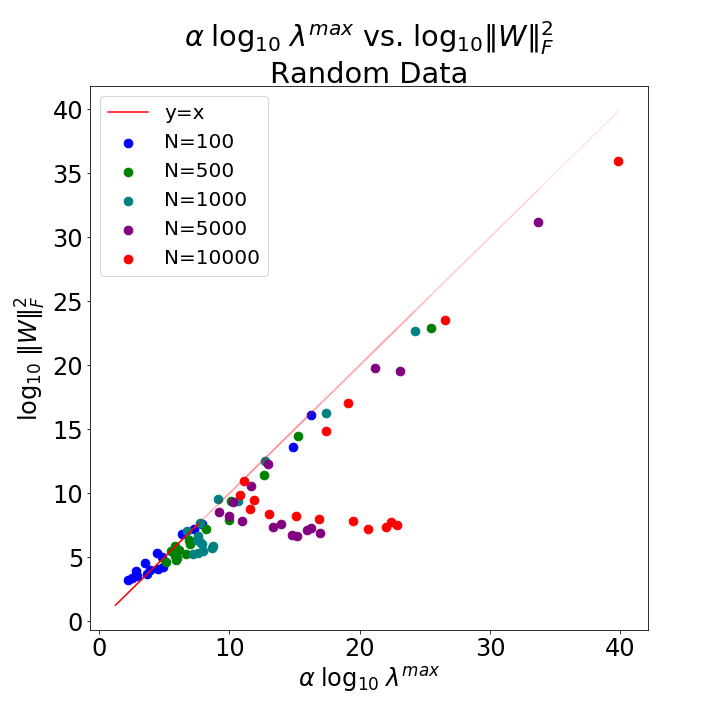
\includegraphics[scale=0.30]{img/relation-rand.png} 
        \label{fig:relation-rand}
    }
    \subfigure[VGG11 Weight matrices]{
        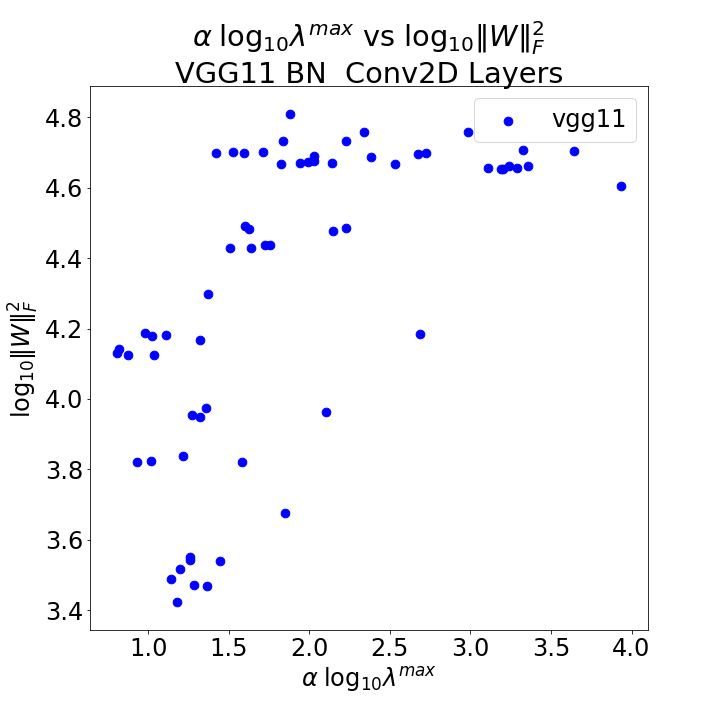
\includegraphics[scale=0.30]{img/relation-vgg11.png} 
        \label{fig:relation-vgg11}
    }
        \caption{Relation between $\alpha\log_{10}\lambda_{max}$ and $\log_{10}\Vert\mathbf{W}\Vert^{2}_{F}$ for random (Pareto) matrices and real (VGG11) DNN weight matrices.
                 \michael{Charles, change $M$ to $N$ in caption.}
                 }
    \label{fig:relations}
\end{figure}

Here, we show numerically that the qualitative form of Eqn.~(\ref{eqn:basic_relation}) holds more generally than the special case derived previously, including into the MHT Universality class, for both random and real data.
To illustrate this, we generate a large number of HT random matrices $\mathbf{W}^{rand}(\mu)$, with varying sizes $N$ (with, for simplicity, aspect ratio $Q=1$), drawn from a Pareto distribution of Eqn.~(\ref{eqn:ht_dstbn}), with exponents $\mu\in[0.5, 5]$.
We then fit the ESD of each $\mathbf{W}^{rand}(\mu)$ to a PL using the method of Clauset et al.~\cite{CSN09_powerlaw,ABP14} to obtain the empirical exponent $\alpha$.   
Figure~\ref{fig:relation-rand} shows that there is a near-perfect relation between $ \alpha\log\lambda_{max}$ and $\log\Vert\mathbf{W}\Vert^{2}_{F} $.
We also performed a similar PL fit for VGG11 weight matrices.
(See Section~\ref{sxn:emp} for some details on the VGG11 model.)
Figure~\ref{fig:relation-vgg11} shows the results, demonstrating an increasing relation until $ \alpha\log\lambda_{max} \approx 2.5$ and a saturation after that point.
Figure~\ref{fig:relations} illustrates
(among other things\footnote{Clearly, there are also differences between the HT random and the real DNN matrices, most notably that $ \alpha\log\lambda_{max} $ achieves much larger values for the random matrices.  This is discussed in more detail in Appendix~\ref{sxn:appendix-universality}.})
that multiplying $\alpha$ by $\log_{10}\lambda_{max}$ leads to a relation that increases linearly with the (log of the squared) Frobenius norm for HT random matrices, and that the two quantities are linearly correlated for real DNN weight matrices.

%% \michael{Maybe comment also about how points large on the X axis have smaller $\alpha$.}
%% 
%% \charlesX{LEAD INTO HOW WE GOT THIS SECTION... PRESENT THE PL-NORM RELATION, SHOW THAT IT IS THE RIGHT SLOPE, AND HOW THE FINITE SIZE  EFFECTS LET US EXTEND THIS RELATION ACROSS UNIVERSALITY CLASSES IN ROUGH WAY, GIVING A USEFUL METRIC FOR ENGINEERING WORK.  REAL DATA IS SHOWN.  HAS 4 PLOTS.  USES NUMERICAL METHODS DESCRIBED ABOVE.  WE MAY WANT PSEUDOCODE ALSO ?}


\paragraph{The PL--Norm Relation: Finite-Size Effects.}


\begin{figure}[t] %[!htb]
   \centering
   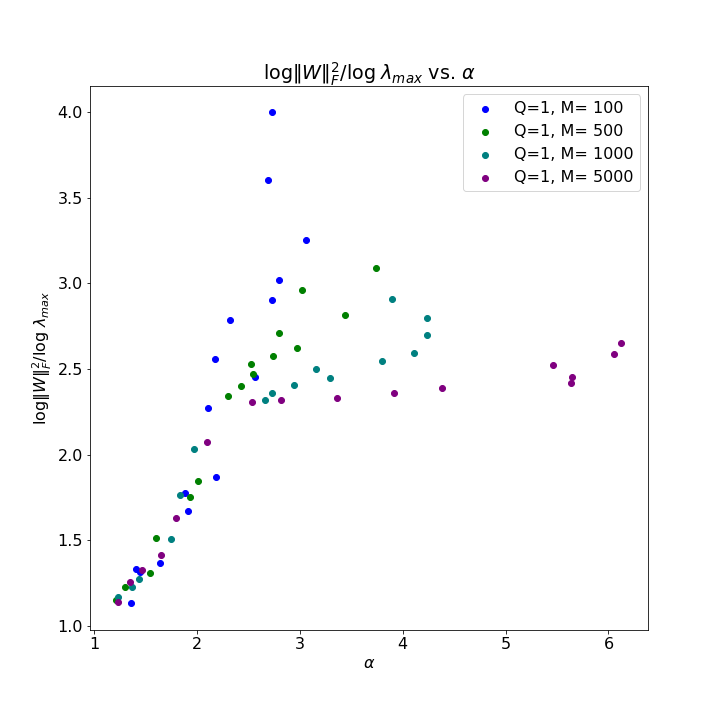
\includegraphics[scale=0.30]{img/Alpha-LogNorm-Relations.png}
   \caption{
            Numerical test of Eqn.~(\ref{eqn:basic_relation}) for random HT matrices across different HT Universality classes.
            \michael{Charles, change $M$ to $N$ in caption.}
           }
   \label{fig:randW}
\end{figure}

Here, we consider finite-size effects in Eqn.~(\ref{eqn:basic_relation}), both within and across HT Universality classes, i.e., for both VHT and MHT matrices.
See Figure~\ref{fig:randW}, which  displays $\frac{\log\Vert\mathbf{W}\Vert^{2}_{F}}{\log\lambda_{max}}$ as a function of the fitted PL exponent $\alpha$, with varying sizes $N$ (with, for simplicity, aspect ratio $Q=1$).
Recall that $\alpha \approx \frac{1}{2}\mu+1$ for finite-sized VHT random matrices, while $\alpha = a\mu+b$ for finite-sized MHT random matrices, where $a,b$ depend strongly on the size of the matrix.  Thus, $\mu\in(0,2)$ for VHT matrices corresponds to $\alpha\in(1,2)$, while $\alpha \approx(2,3)$ or $\alpha \approx(2,4)$ for MHT matrices.
%% $$
%% \dfrac{\log\Vert\mathbf{W}\Vert^{2}_{F}}{\log\lambda_{max}}\;\;vs.\;\;(\alpha)  .
%% $$
The numerical results in Figure~\ref{fig:randW} show that as $\alpha$ increases:
when $\alpha<2$, there exists a near-linear relation; and
when $\alpha>2$, for $N,M$ large, the relation saturates, becoming constant, while for smaller $N,M$, there exists a near-linear relation, but with strong finite-size effects.
These numerical results demonstrate that $ \log\Vert\mathbf{W}\Vert^{2}_{F}\approx\alpha\log\lambda_{max} $ works very well for VHT random matrices, for $\alpha<2$, and that it works moderately well for MHT matrices and even some WHT matrices.
In particular, for MHT matrices, the finite-size regime in which it holds moderately well is when $N,M$ is on the order of a hundred to a thousand, which is a typical value for modern DNNs. 

%% \michael{Make sure what I include in the above par is enough for what I need here.}
%% \michael{Here is the place to make explicit the connection between $\alpha$ and $\mu$, for finite $N$ and asymptotically, and to say Eqns.~(\ref{eqn:alpha_mu_vht_and_mht}) holds for both VHT and MHT, for realistic values of $N$.}

%To understand this relation better, and to sketch a proof,
%we will generate the data for a number of a Heavy-Tailed random matrices, 
%with different power law exponents $\mu$.
%Note that this linear relation holds over several log scales.  However,
%the relation does deviate from linearity at the smaller values of $\alpha\;\log_{10}\;\lambda_{max}$.
%This is readily explained below .  


%%MM%% This approximate relation formally only hold in the asymptotic limit of very small power law exponents $\alpha\rightarrow 1$ for
%%MM%% random heavy tailed matrices, but using Universality, we can safely extend it up to the finite-size MHT class, with
%%MM%% exponents $\alpha=4$ (and larger).  


